\scanpage{4}
% The upper right arrow is heavily retraced; its earlier direction is not recoverable.

\diagram{\begin{tikzcd}[ampersand replacement=\&,column sep=1.6em,row sep=1.2ex]
\mathrm{Ob}\,C_4\arrow[rr,line width=.8pt]\arrow[rr,bend left=7,dash]\arrow[rr,bend right=3,dash] \& \& \mathrm{Fl}_0(\unsure{C_1|C_n})\\
{\tikz[baseline=(topproduct.base)]{
 \node[inner sep=0pt] (topproduct) {\(\bigl(\mathbb F\mathrm l\,C_1\times\mathrm{Ob}\,C_2\bigr)\)};
 % Small detached ink fleck below/right of F; affiliation is uncertain.
 \fill ([xshift=1.05em,yshift=-.48em]topproduct.west) circle[radius=.025em];}}
 \arrow[u,shift left=.55ex]\arrow[u,shift right=.55ex]
 \& {\deleted{\amalg}\;\deleted{\unsure{\mathrm{Fl}_0 C_1\times}}\;
 \inserted{\mathbb F\mathrm l_0(C_1)\times\mathrm{Ob}\,C_2}} \&
\end{tikzcd}}

\[
\mathbb F\mathrm l\,C_{\deleted{\unsure{2}}\unsure{1|2}}\times
\mathbb F\mathrm l(C_2)\times\deleted{\unsure{\mathrm{Fl}|F}}\mathrm{Ob}\,C_3
\]

\figure{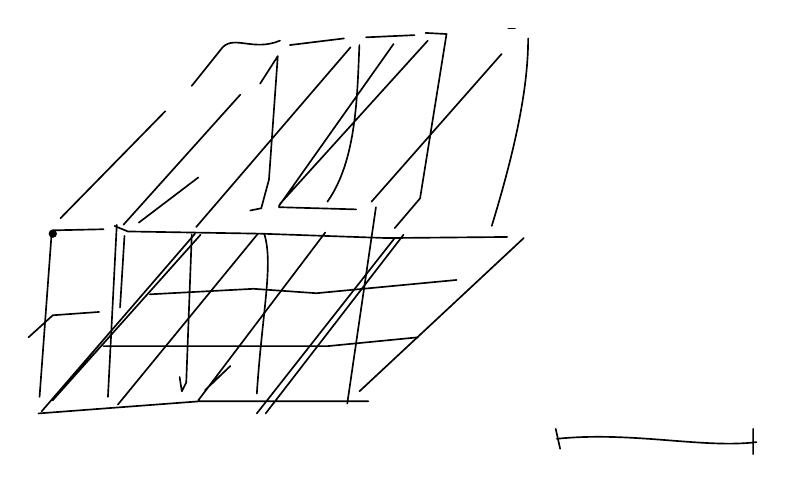
\begin{tikzpicture}[x=.014cm,y=-.014cm,line width=.6pt,line cap=round,line join=round]
\draw (1305,284)--(1351,283) (1361,280)--(1373,285)--(1493,287)--(1608,291)--(1717,290)
 (1304,286)--(1293,435) (1363,279)--(1355,435) (1370,289)--(1366,354)
 (1431,288)--(1426,422)--(1422,430)--(1420,417)
 (1497,288)..controls(1505,316)and(1495,357)..(1490,432) (1598,263)--(1572,441);
\draw (1292,450)--(1438,439)--(1591,439)
 (1295,448)--(1434,287) (1305,438)--(1439,288)
 (1364,442)--(1491,287) (1437,438)--(1552,286) (1443,429)--(1466,407)
 (1490,450)--(1615,291) (1498,450)--(1623,288) (1583,430)--(1732,291);
\draw (1283,381)--(1305,361)--(1347,358) (1351,389)--(1554,389)--(1636,381)
 (1393,342)--(1487,337)--(1544,341)--(1671,329);
\draw (1312,273)--(1407,176) (1369,279)--(1475,161) (1383,277)--(1437,236)
 (1431,153)--(1459,118)..controls(1470,107)and(1487,122)..(1511,112)
 (1493,151)--(1509,126)--(1501,238)--(1494,264)--(1484,266)
 (1520,116)--(1569,110) (1435,281)--(1575,118)
 (1510,262)--(1614,115) (1510,263)--(1580,265)
 (1554,258)..controls(1581,220)and(1581,159)..(1583,116)
 (1589,109)--(1633,107) (1511,260)--(1645,112)
 (1643,105)--(1662,106)--(1638,255)--(1615,282)
 (1594,258)--(1712,124) (1703,280)..controls(1725,208)and(1736,154)..(1736,110);
\draw (1718,101)--(1724,101);
\fill (1305,287) circle[radius=3.8];
\draw (1762,473)..controls(1830,466)and(1895,482)..(1943,476)
 (1761,464)--(1765,482) (1940,464)--(1940,487);
\end{tikzpicture}}

\[
\mathbb F_3=\mathrm{Fl}\,C_1\times\mathrm{Fl}\,C_2
\,\unsure{<|\times}\,\mathrm{Fl}\,\ell_3\times\mathrm{Ob}\,C_4
\]

\[
\mathbb F_n\mathrel{\unsure{2|=}}
\tikz[baseline=(nfirstfactor.base)]{\node[inner sep=0pt] (nfirstfactor) {\(\mathbb F\mathrm l\,C_1\)};
 % Detached dark fleck just before C, without an assigned mathematical role.
 \fill ([xshift=1.47em,yshift=-.23em]nfirstfactor.west) circle[radius=.025em];}
\times\mathrm{Fl}\,C_2\ \text{---}\ \times\mathrm{Fl}\,C_n
\deleted{\times\mathrm{Ob}\,C_4}
\]

\figure{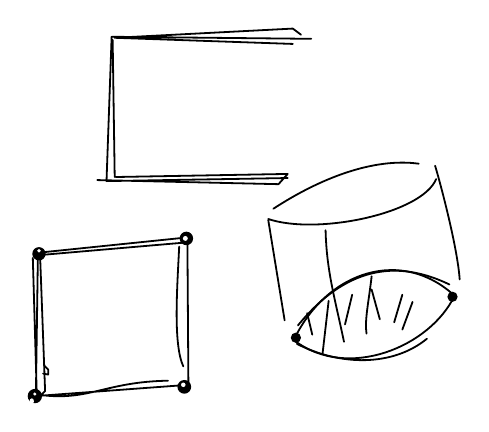
\begin{tikzpicture}[x=.013cm,y=-.013cm,line width=.65pt,line cap=round,line join=round]
\draw (1805,608)--(1610,606)--(1605,747)--(1782,744)
 (1795,604)--(1787,598)--(1613,607)--(1787,613)
 (1611,609)--(1613,743) (1596,746)--(1773,750)--(1782,740)--(1614,743);
\draw (1538,817)--(1684,802)--(1685,946)--(1536,957)--cycle
 (1543,819)--(1682,807) (1533,822)--(1537,960)--(1545,952)--(1540,817)
 (1676,811)..controls(1674,852)and(1670,906)..(1680,928)
 (1541,956)..controls(1588,962)and(1604,943)..(1665,942);
\fill (1539,818) circle[radius=6.5] (1683,803) circle[radius=6.6]
 (1681,948) circle[radius=6.7] (1535,957) circle[radius=7];
\fill[white] (1539,815) circle[radius=1.8] (1682,803) circle[radius=2.4]
 (1680,946) circle[radius=2.2] (1535,955) circle[radius=1.6];
\fill[white] (1532,962) ellipse[x radius=2.1,y radius=2.8];
\draw (1544,927)--(1548,931)--(1548,936)--(1543,935);
\draw (1768,774)..controls(1814,744)and(1866,724)..(1910,730)
 (1763,784)..controls(1810,800)and(1913,779)..(1927,745)
 (1763,785)--(1779,883) (1926,732)..controls(1932,752)and(1948,813)..(1950,843)
 (1819,795)..controls(1820,835)and(1828,861)..(1837,904);
\draw (1789,900)..controls(1822,834)and(1894,812)..(1945,859)
 ..controls(1921,909)and(1841,942)..(1789,903);
\draw (1792,888)..controls(1832,839)and(1880,819)..(1940,848)
 (1791,906)..controls(1834,928)and(1885,928)..(1918,901);
\draw (1801,876)--(1806,897) (1822,864)--(1816,916) (1845,858)--(1838,887)
 (1864,840)..controls(1861,866)and(1857,883)..(1859,896)
 (1864,853)--(1872,882) (1894,858)--(1886,885) (1904,865)--(1894,892);
\fill (1790,900) circle[radius=5] (1943,860) circle[radius=5];
\end{tikzpicture}}

\[
\tikz[baseline=(markletters.base)]{
 \node[inner sep=0pt] (markletters) {\(\unsure{X_0|X_{\varnothing}}\qquad X_1\)};
 \draw[line width=.32pt] ([xshift=.39em,yshift=-.08em]markletters.west)
 ..controls ([xshift=.25em,yshift=-.80em]markletters.west) and ([xshift=.87em,yshift=-.55em]markletters.west)
 ..([xshift=1.13em,yshift=-.31em]markletters.west)
 ..controls ([xshift=2.00em,yshift=.55em]markletters.west) and ([xshift=-1.48em,yshift=.55em]markletters.east)
 ..([xshift=-1.43em,yshift=-.05em]markletters.east)
 ..controls ([xshift=-1.43em,yshift=-.55em]markletters.east) and ([xshift=-.79em,yshift=-.42em]markletters.east)
 ..([xshift=-.32em,yshift=.08em]markletters.east);
 % The short parallel rising stroke and detached fleck are visible ink.
 \draw[line width=.25pt] ([xshift=.48em,yshift=.09em]markletters.west)--([xshift=.69em,yshift=.40em]markletters.west);
 \fill ([xshift=-1.63em,yshift=.77em]markletters.east) circle[radius=.025em];}
\]

\[
\bullet\quad O_1\subset\mathbb F_1\qquad
\deleted{\mathbb F}O_2\subset\mathbb F_2\quad\text{---}\quad O_n\subset\mathbb F_n
\]

\[
\deleted{O}\hat F\subset\mathbb F
\]

\[
\mathbb F_1\times\text{---}\ 
% Literal multiplication-stroke traces retain detached ink; no prime is inferred.
\mathbin{\tikz[baseline={([yshift=-.45ex]current bounding box.center)},x=.013cm,y=-.013cm,line width=.35pt,line cap=round]{
 \draw (824,1219)--(841,1236) (824,1234)--(843,1214);
 \draw (837,1199)..controls(840,1201)and(838,1205)..(837,1207);
 \draw (826,1215)--(829,1218);}}
\mathbb F_n
\mathbin{\tikz[baseline={([yshift=-.45ex]current bounding box.center)},x=.013cm,y=-.013cm,line width=.35pt,line cap=round]{
 \draw (952,1206)--(983,1237) (955,1236)--(973,1206);
 \fill (977,1198) circle[radius=1.3];}}
(-\,?)
\]

\[
(O_1,\mathbb F_1)\mathbin{*}(O_2,\mathbb F_2)\ \text{---}\mathbin{*}
(\deleted{\unsure{O|0}}\unsure{O_3|O_n}\,\unsure{F_{n+1}|F_n|F_3})\,.
\]

\figure{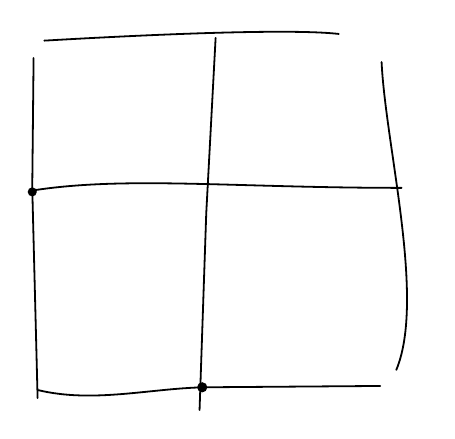
\begin{tikzpicture}[x=.017cm,y=-.017cm,line width=.65pt,line cap=round]
\draw (1374,1202)..controls(1460,1197)and(1559,1193)..(1594,1197)
 (1366,1215)--(1365,1312)--(1369,1469)
 (1365,1314)..controls(1435,1303)and(1515,1312)..(1641,1312)
 (1502,1200)--(1495,1331)--(1490,1478)
 (1369,1463)..controls(1410,1473)and(1452,1462)..(1493,1461)--(1625,1460)
 (1626,1218)..controls(1629,1281)and(1659,1395)..(1637,1448);
\fill (1365,1315) circle[radius=3.4] (1492,1461) circle[radius=3.8];
\end{tikzpicture}}

\[
(F\times I)\mathbin{\amalg}_{\deleted{O}\dot F\times I}\deleted{O}\hat F
\]
% archive sheet number: 3
